\documentclass{algblatt}
\usepackage{tikz}
\usepackage{pdfpages}
\loesungenfalse

\geometry{tmargin=2.0cm,bmargin=2.0cm,lmargin=2.25cm,rmargin=2.25cm}

%\setlength{\titleskip}{0.7em}
\setlength{\aufgabenskip}{1.0em}

\begin{document}

\vspace*{-1.5cm}
\maketitle{13}{Abgabe bis 15. Juli 2013, 17:00 Uhr}

\begin{aufgabe}{Konstruierbare~$n$-Ecke}
\begin{enumerate}
\item Für welche~$n \in \{ 1,\ldots,100 \}$ ist ein regelmäßiges~$n$-Eck
mit Zirkel und Lineal konstruierbar?
\item Gib eine Konstruktionsvorschrift für das regelmäßige~$15$-Eck an.
\end{enumerate}

\begin{loesungE}
\item Satz~4.30 gibt die Antwort vor: Es sind genau die~$n$-Ecke konstruierbar,
für die~$n$ von der Form~$2^r p_1 \cdots p_s$, $r,s \geq 0$ sind, wobei
die~$p_i$ paarweise verschiedene Fermatsche Primzahlen sind -- das sind
Primzahlen, die von der Form~$F_k = 2^{2^k} + 1$, $k \geq 0$, sind. Die ersten
vier Fermatschen Primzahlen sind
\[ F_0 = 3,\quad
  F_1 = 5,\quad
  F_2 = 17,\quad
  F_3 = 257. \]
(Es sind aber nicht alle~$F_k$ Primzahlen, etwa ist~$F_5$ durch~$631$ teilbar.)

Für~$n \leq 100$ sind nur die ersten drei Fermatschen Primzahlen relevant; es
ergibt sich, dass genau folgende~$n$-Ecke mit~$n \geq 100$ konstruierbar
sind:
\[ 1,2,3,4,5,6,8,10,12,15,16,17,20,24,30,32,34,40,48,51,60,64,68,80,85,96. \]
Das sind insgesamt~26 Stück.

\item Ich bin gerade zu faul zum Zeichnen und binde auf der nächsten Seite eine
detaillierte Konstruktionsbeschreibung von
\url{http://www.walser-h-m.ch/hans/Miniaturen/1/15-Eck/15-Eck.pdf} ein.
\end{loesungE}
\end{aufgabe}
\ifloesungen
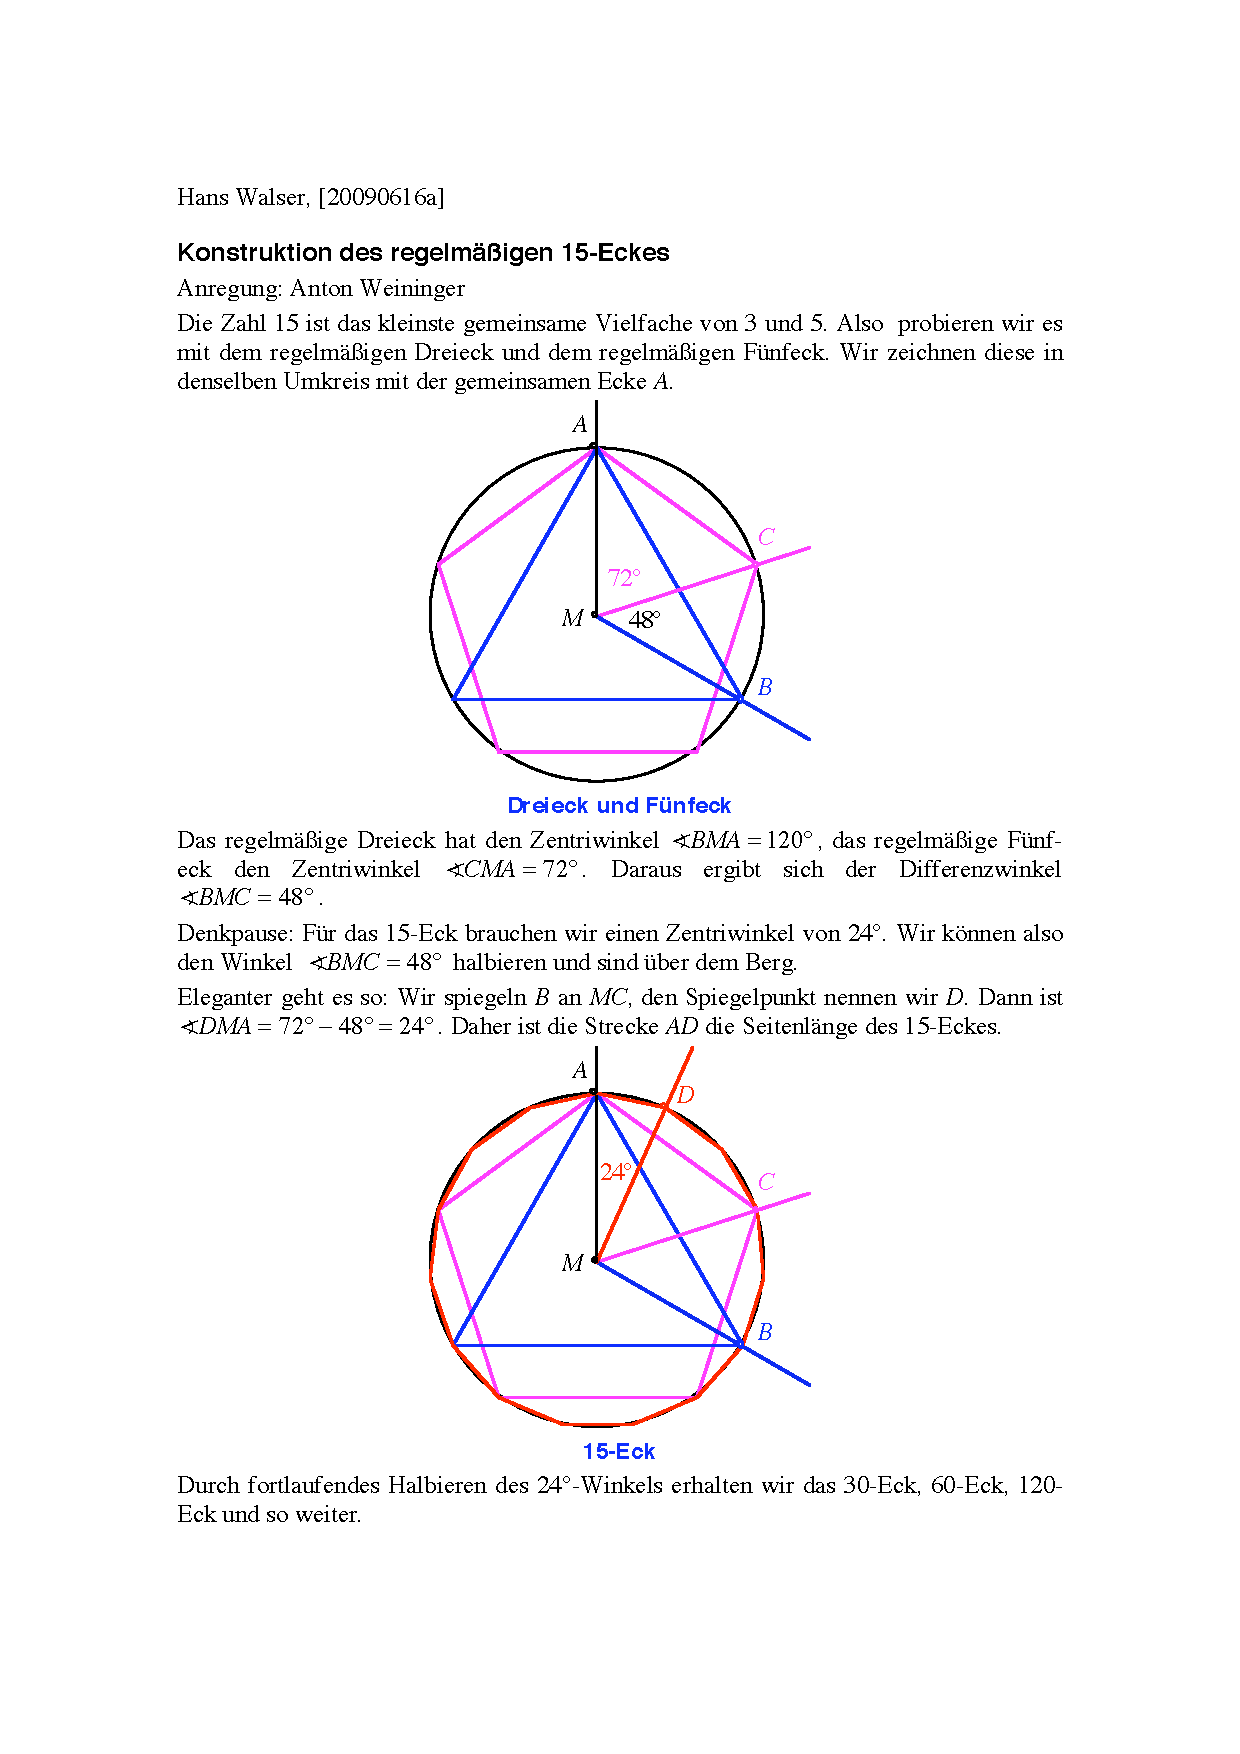
\includepdf{15-Eck}
\fi

\begin{aufgabe}{Fermatsche und Mersennesche Primzahlen}
\begin{enumerate}
\item Zeige für alle natürlichen Zahlen~$n \geq 0$: $F_{n+1} = 2 + F_n F_{n-1}
\cdots F_0$.
\item Zeige, dass~$F_m$ und~$F_n$ für~$m \neq n$ teilerfremd sind. Folgere
daraus, dass es unendlich viele Primzahlen gibt.
\item Eine \emph{Mersennesche Zahl} ist eine Zahl der Form~$M_n = 2^n -
1$. Zeige, dass~$M_n$ höchstens dann eine Primzahl ist, wenn~$n$ eine Primzahl
ist.
\item Zeige allgemeiner, dass~$M_n$ von~$M_d$ geteilt wird, wenn~$d$ ein
positiver Teiler von~$n$ ist.
\end{enumerate}

\begin{loesungE}
\item Per Definition ist~$F_k = 2^{2^k} + 1$. Die Konvention ist so,
dass~$2^{(2^k)}$ und nicht~$(2^2)^k = 4^k$ gemeint ist. Die Behauptung zeigen
wir durch einen Induktionsbeweis. Für~$n = 0$ ist die Aussage klar:
\[ F_{0+1} = 5 = 2 + 3 = 2 + F_0. \]
Für den Schritt~$n \to n + 1$ rechnen wir:
\begin{align*}
  2 + F_{n+1} F_n F_{n-1} \cdots F_0 &=
  2 + F_{n+1} \cdot (F_n F_{n-1} \cdots F_0 + 2 - 2) \\
  &\stackrel{\text{IV}}{=} 2 + F_{n+1} \cdot (F_{n+1} - 2)
  = (F_{n+1} - 1)^2 + 1 \\
  &= \bigl(2^{2^{n+1}}\bigr)^2 + 1
  = 2^{2^{n+2}} + 1
  = F_{n+2}.
\end{align*}

\item Ohne Einschränkung sei~$m > n$. Sei~$d$ ein gemeinsamer Faktor von~$F_m$
und~$F_n$. Aus Teilaufgabe~a) kennen wir die Beziehung
\[ F_m = F_{(m-1)+1} = 2 + F_{m-1} \cdots F_0. \]
Der hintere Summand ist ein Vielfaches von~$d$, da einer der Faktoren~$F_n$
ist. Daher folgt, dass auch~$2$ ein Vielfaches von~$d$ ist; der Teiler~$d$ ist
also~$\pm 1$ oder~$\pm 2$. Letzteres kann aber nicht eintreten: Direkt an der
Form der fermatschen Zahlen erkennt man, dass~$\pm 2$ kein Teiler von ihnen
ist. Also ist~$d = \pm 1$. Das war zu zeigen.

Eine unendliche Folge paarweise verschiedener Primzahlen können wir mit dieser
Erkenntnis wie folgt konstruieren: Wir zerlegen sukzessive die
Zahlen~$F_0,F_1,\ldots$ in Primfaktoren. Diese Primfaktoren werden wegen der
Teilerfremdheit alle unterschiedlich sein. Somit erhalten wir also beliebig
viele paarweise verschiedene Primzahlen.

\emph{Bemerkung:} Der Beweis stammt von Goldbach. In der Praxis ist er
allerdings ein recht umständliches Verfahren zur Primzahlgenerierung, da
die~$F_n$ rasant groß werden:
\begin{align*}
  F_0 &= 3 \\
  F_1 &= 5 \\
  F_2 &= 17 \\
  F_3 &= 257 \\
  F_4 &= 65537 \\
  F_5 &= 4294967297 = 641 \cdot 6700417 \\
  F_6 &= 18446744073709551617 = 274177 \cdot 67280421310721
\end{align*}
Es ist ein offenes Forschungsproblem, ob~$F_{33}$ eine Primzahl ist.

\item Wir zeigen: Ist~$n$ eine zusammengesetzte Zahl, so auch~$M_n$. Sei
dazu~$n = a \cdot b$ eine Zerlegung mit~$a,b \geq 2$. Dann folgt
\begin{align*}
  M_n &= 2^n - 1 = 2^{ab} - 1 = (2^a)^b - 1 \\
  &= (2^a - 1) \cdot (1 + 2^a + (2^a)^2 + \cdots + (2^a)^{b-1}).
\end{align*}
Da~$a,b \geq 2$, folgt~$2^a - 1 \geq 2^2 - 1 = 3$ und~$\text{(hinterer Faktor)}
\geq 1 + 2^a \geq 1 + 2^2 = 5$, also ist diese Zerlegung von~$M_n$ eine echte
und~$M_n$ somit zusammengesetzt.

\item Gelte~$n = d \cdot \ell$. Dann folgt völlig analog (sogar identisch!)
\begin{align*}
  M_n &= 2^n - 1 = 2^{d\ell} - 1 = (2^d)^\ell - 1 \\
  &= (2^d - 1) \cdot (1 + 2^d + (2^d)^2 + \cdots + (2^d)^{\ell-1}),
\end{align*}
also ist~$M_d = 2^d - 1$ ein Teiler von~$M_n$.
\end{loesungE}
\end{aufgabe}

\begin{aufgabe}{Hauptsatz der Galoistheorie}
Bestimme alle Untergruppen der galoisschen Gruppe der Nullstellen des
Polynoms~$X^4 + 1$ und die zugehörigen Zwischenerweiterungen.

\begin{loesung}
In Aufgabe~3 von Blatt 10 haben wir die Galoisgruppe bereits berechnet: Es
gilt~$\QQ(x_1,x_2,x_3,x_4) = \QQ(t)$ mit~$t = \xi := \exp(2\pi\i/8)$ und
\[ \Gal_\QQ(x_1,x_2,x_3,x_4) =
  \left\{ \id, \sigma, \tau, \mu \right\} \]
mit
\begin{align*}
  \sigma &= (1,2)\circ(3,4), \\
  \tau &= (1,3)\circ(2,4), \\
  \mu &= (1,4)\circ(2,3).
\end{align*}
\begin{itemize}
\item Untergruppen der Ordnung~1: $U_1 = \{\id\}$.
\item Untergruppen der Ordnung~2: $U_2 = \{\id,\sigma\}$, $U_3 = \{\id,\tau\}$,
$U_4 = \{\id,\mu\}$.
\item Untergruppen der Ordnung~3: Kann es keine geben (Lagrange!).
\item Untergruppen der Ordnung~4: $U_5 = \{\id,\sigma,\tau,\mu\}$.
\end{itemize}
Die zugehörigen Zwischenerweiterungen sind laut der expliziten Formel aus
Proposition~5.9:
\begin{align*}
  \QQ(t)^{U_1} &= \QQ(t) \\
  \QQ(t)^{U_2} &= \QQ(t + \sigma(t), t \cdot \sigma(t)) =
    \QQ(\xi + \xi^3, \xi \cdot \xi^3) =
    \QQ(\sqrt{2}\,\i, -1) =
    \QQ(\sqrt{2}\,\i) \\
  \QQ(t)^{U_3} &= \QQ(t + \tau(t), t \cdot \tau(t)) =
    \QQ(\xi + \xi^5, \xi \cdot \xi^5) =
    \QQ(0, -\i) = \QQ(\i) \\
  \QQ(t)^{U_4} &= \QQ(t + \mu(t), t \cdot \mu(t)) =
    \QQ(\xi + \xi^7, \xi \cdot \xi^7) =
    \QQ(\sqrt{2}, 1) =
    \QQ(\sqrt{2}) \\
  \QQ(t)^{U_5} &= \QQ
\end{align*}
Die Zwischenerweiterungs- und Untergruppendiagramme sehen also wie folgt aus:
\begin{center}\begin{tikzpicture}[node distance=2cm]
 \node (Q)                  {$\mathbb{Q}$};
 \node (Q6)  [above of=Q]   {$\mathbb{Q}(\i)$};
 \node (Q2)  [right of=Q6]  {$\mathbb{Q}(\sqrt{2})$};
 \node (Q3)  [left of=Q6]   {$\mathbb{Q}(\sqrt{2}\,\i)$};
 \node (Q23) [above of=Q6]  {$\mathbb{Q}(\xi)$};
 \node (1f)  [right of=Q2]  {$\{\id,\sigma\}$};
 \node (1fg) [right of=1f]  {$\{\id,\tau\}$};
 \node (1g)  [right of=1fg] {$\{\id,\mu\}$};
 \node (G)   [below of=1fg] {$\{\id,\sigma,\tau,\mu\}$};
 \node (1)   [above of=1fg] {$\{\id\}$};
 \draw (Q)   -- (Q2);
 \draw (Q)   -- (Q3);
 \draw (Q)   -- (Q6);
 \draw (Q2)  -- (Q23);
 \draw (Q3)  -- (Q23);
 \draw (Q6)  -- (Q23);
 \draw (G)   -- (1f);
 \draw (G)   -- (1fg);
 \draw (G)   -- (1g);
 \draw (1f)  -- (1);
 \draw (1fg) -- (1);
 \draw (1g)  -- (1);
\end{tikzpicture}\end{center}
Links markiert man üblicherweise die Striche mit den zugehörigen Graden, rechts
mit den zugehörigen Indizes. Diese sind hier alle jeweils~$2$.
\end{loesung}
\end{aufgabe}

\begin{aufgabe}{Relative galoissch Konjugierte}
\begin{enumerate}
\item Finde zwei algebraische Zahlen, die über~$\QQ$ galoissch konjugiert sind,
über~$\QQ(\sqrt{3})$ aber nicht.
\item Seien~$K$ und~$L$ Koeffizientenbereiche mit~$L \supseteq K \supseteq
\QQ$ und~$x$ eine algebraische Zahl. Zeige, dass ein galoissch Konjugiertes
von~$x$ über~$L$ auch ein galoissch Konjugiertes von~$x$ über~$K$ ist.
\end{enumerate}

\begin{loesungE}
\item Ein Beispiel bilden die Zahlen~$\pm\sqrt{3}$. Diese sind über~$\QQ$
sicherlich zueinander galoissch konjugiert (ihr gemeinsames Minimalpolynom
ist~$X^2 - 3$), aber über~$\QQ(\sqrt{3})$ haben sie verschiedene
Minimalpolynome~(nämlich~$X \mp \sqrt{3}$).

\item Seien~$m_K$ und~$m_L$ die Minimalpolynome von~$x$ über~$K$ bzw.~$L$. Wenn
wir~$m_K$ als Polynom über~$L$ auffassen, sagt uns der abelsche
Irreduzibilitätssatz, dass~$m_L$ ein Teiler von~$m_K$ sein muss (über~$L$) --
denn~$m_K$ und~$m_L$ haben die gemeinsame Nullstelle~$x$ und~$m_L$ ist
irreduzibel über~$L$. Folglich ist jede Nullstelle von~$m_L$, also jedes
galoissch Konjugierte von~$x$ über~$L$, auch eine Nullstelle von~$m_K$, also
ein galoissch Konjugiertes von~$x$ über~$K$.
\end{loesungE}
\end{aufgabe}

\begin{aufgabe}{Relative Galoisgruppen}
\begin{enumerate}
\item Finde ein normiertes separables Polynom mit rationalen Koeffizienten,
sodass die galoissche Gruppe seiner Nullstellen über~$\QQ$ gleich der
über~$\QQ(\sqrt[3]{5})$ ist.
\item Sei~$f \in K[X]$ ein normiertes separables Polynom und~$x_1,\ldots,x_n$
seine Nullstellen. \\ Sei~$y \in K(x_1,\ldots,x_n)$. Zeige:
\[ \Gal_{K(y)}(x_1,\ldots,x_n) = \{ \sigma \in \Gal_K(x_1,\ldots,x_n) \,|\,
\sigma \cdot y = y \}. \]
\end{enumerate}

\begin{loesungE}
\item Ein Beispiel ist das Polynom~$X - 1$. 

\item "`$\subseteq$"': Sei~$\sigma \in \Gal_{K(y)}$ beliebig. Dann
erhält~$\sigma$ also alle algebraischen Relationen zwischen den Nullstellen mit
Koeffizienten aus~$K(y)$; insbesondere erhält~$\sigma$ also alle algebraischen
Relationen mit Koeffizienten aus~$K$, daher liegt~$\sigma$ auch in~$\Gal_K$.

Ferner muss~$\sigma$ das Element~$y$ festlassen: Vielleicht findet man das
offensichtlich (da die Galoisgruppe über~$K(y)$ nach Vorlesung trivial
auf~$K(y)$ operiert), eine explizite Begründung kann man aber auch formulieren:
Da~$y \in K(x_1,\ldots,x_n)$, gibt es ein Polynom~$H \in K[X_1,\ldots,X_n]$
mit~$H(x_1,\ldots,x_n) = y$. Das Polynom~$H(X_1,\ldots,X_n) - y \in
K(y)[X_1,\ldots,X_n]$ ist eine algebraische Relation der Nullstellen
über~$K(y)$ und wird daher von~$\sigma$ erhalten -- es gilt also
\[ 0 = H(x_{\sigma(1)},\ldots,x_{\sigma(n)}) - y = \sigma \cdot y - y. \]

"`$\supseteq$"': Sei~$\sigma \in \Gal_K$ mit~$\sigma \cdot y = y$ beliebig.
Um~$\sigma \in \Gal_{K(y)}$ nachzuweisen, müssen wir zeigen, dass jede algebraische
Relation~$H \in K(y)[X_1,\ldots,X_n]$ der Nullstellen über~$K(y)$
unter~$\sigma$ erhalten bleibt. Dazu rechnen wir:
\begin{align*}
  H(x_{\sigma(1)},\ldots,x_{\sigma(n)}) &=
  H(\sigma \cdot x_1,\ldots,\sigma \cdot x_n) =
  (\sigma \cdot H)(\sigma \cdot x_1,\ldots,\sigma \cdot x_n) \\
  &= \sigma \cdot H(x_1,\ldots,x_n) = \sigma \cdot 0 = 0.
\end{align*}
Dabei ging beim zweiten Gleichheitszeichen die Voraussetzung~$\sigma \cdot y =
y$ ein. Beim dritten Gleichheitszeichen haben wir die Additivität und
Multiplikativität der Wirkung von~$\sigma$ verwendet: Ausgeschrieben steht ein
langer Ausdruck da, dessen Teile alle von~$\sigma$ umklammert werden. Dieses
kann man vor den gesamten Term ziehen.
\end{loesungE}
\end{aufgabe}

\begin{aufgabe}{Zentrum einer Galoisgruppe}
Sei~$p$ eine Primzahl und~$x$ eine algebraische Zahl vom Grad~$p^n$. Seien alle
galoissch Konjugierten~$x_1 = x, x_2, \ldots, x_{p^n}$ von~$x$ in~$x$ rational.
\begin{enumerate}
\item Zeige, dass das Zentrum der galoisschen Gruppe der~$x_1,\ldots,x_{p^n}$ ein
Element~$\sigma$ der Ordnung~$p$ enthält.
\item Sei~$\sigma$ eine Permutation wie in~a) und~$y$ ein primitives Element
zu den Zahlen~$e_i(x_1,\sigma\cdot x_1,\ldots,\sigma^{p-1}\cdot x_1)$, $i =
1,\ldots,p$. Zeige, dass~$y$ vom Grad~$p^{n-1}$ ist.
\end{enumerate}

\begin{loesungE}
\item Die Anzahl der Elemente der Galoisgruppe ist eine~$p$-Potenz:
\[ |\Gal_\QQ(x_1,\ldots,x_{p^n})| = \gra{\QQ(x_1,\ldots,x_{p^n})}{\QQ} =
\gra{\QQ(x)}{\QQ} = p^n. \]
Nach Proposition~4.24 gibt es daher ein Element der Ordnung~$p$ im Zentrum.

\item \emph{Schritt 1:}
Wir sollten uns zunächst ein wenig Übersicht verschaffen. Da die Ordnung
der Permutation~$\sigma$ die Primzahl~$p$ ist, zerfällt~$\sigma$ in lauter
disjunkte~$p$-Zykel. Da~$\sigma$ keine Nullstelle~$x_i$ festhalten darf
(denn~$x_i$ ist nach Proposition~4.4 wie~$x_1$ ein primitives Element --
würde~$\sigma$ daher~$x_i$ festhalten, so würde~$\sigma$ alle Nullstellen
festhalten und wäre somit die Identitätspermutation), kommt sogar \emph{jede} Zahl
aus~$\{1,\ldots,p^n\}$ in einem dieser Zykel vor.

Die Nullstellen~$x_1,\ldots,x_{p^n}$ zerfallen also in~$p^{n-1}$ Blöcke von
je~$p$ Zahlen, die von~$\sigma$ jeweils nur unter sich abgebildet werden. Einer
dieser Blöcke ist
\begin{equation}\label{block}
  x_1, \sigma \cdot x_1, \ldots, \sigma^{p-1} \cdot x_1. \tag{$\star$}
\end{equation}
Die anderen Blöcke erhält man, wenn man statt mit~$x_1$ mit einer anderen
Nullstelle~$x_i$ beginnt (einer, die nicht in diesem Block auftritt).

Wir wollen noch kurz untersuchen, was mit einem solchen Block passiert, wenn
man eine beliebige Symmetrie~$\tau$ der Galoisgruppe auf ihn anwendet:
Da~$\sigma$ (und somit auch~$\sigma^j$) im Zentrum liegt (hier geht diese
Eigenschaft das erste Mal ein), gilt
\[ \tau \cdot (\sigma^j \cdot x_i) = \sigma^j \cdot (\tau \cdot x_i). \]
Die Wirkung von~$\tau$ vertauscht also die Blöcke untereinander.

\emph{Schritt 2:} Da~$y$ ein primitives Element
von~$\QQ(e_1(\star),\ldots,e_p(\star))$ ist, gibt es ein
Polynom~$r \in \QQ[E_1,\ldots,E_p]$ mit~$y = r(e_1(\star),\ldots,e_p(\star))$. Ferner
können wir ein symmetrisches Polynom~$s \in \QQ[Y_1,\ldots,Y_p]$ mit~$y = s(x_1, \sigma
\cdot x_1,\ldots, \sigma^{p-1} \cdot x_1)$ finden. Da~$s$ symmetrisch ist,
ergibt es Sinn, das Polynom
\[ g(X) := \prod (X - s(b_1,\ldots,b_p)) \]
zu definieren, wobei das Produkt über jeden Block~$(b_1,\ldots,b_p)$ genau
einmal gehen soll. Dieses Polynom ist normiert, hat~$y$ als Nullstelle und hat rationale
Koeffizienten -- denn diese sind unter der Wirkung der Galoisgruppe invariant:
Sei~$\tau \in \Gal_\QQ(x_1,\ldots,x_{p^n})$ beliebig. Dann gilt
\[ \tau \cdot g(X) = \prod (X - s(\tau \cdot b_1,\ldots,\tau \cdot b_p)) =
  \prod (X - s(b_1,\ldots,b_p)) = g(X), \]
denn wie wir oben schon gesehen haben, führt~$\tau$ nur zu einer Vertauschung
der Blöcke. Der Grad von~$y$ über~$\QQ$ ist also höchstens gleich dem Grad
von~$g$, und dieser ist~$p^{n-1}$.

\emph{Schritt 3:} Das Polynom
\[ h(X) := \prod_{j=0}^{p-1} (X - \sigma^j \cdot x_1) \]
ist normiert, hat~$x_1$ als Nullstelle und hat Koeffizienten aus~$\QQ(y)$: Denn
diese sind bis auf Vorzeichen durch die elementarsymmetrischen Funktionen in
den~$\sigma^j \cdot x_1$, $j = 0,\ldots,p-1$ gegeben -- und diese sind nach
Voraussetzung rational in~$y$. Folglich ist der Grad von~$x_1$ über~$y$
höchstens~$p$. Somit folgt
\[ \gra{\QQ(y)}{\QQ} = \frac{\gra{\QQ(x_1)}{\QQ}}{\gra{\QQ(x_1)}{\QQ(y)}} \geq
\frac{p^n}{p} = p^{n-1}. \]
Das zeigt die Behauptung.

\emph{Bemerkung:} Mit dem Hauptsatz der Galoistheorie kann man einen
drastisch kürzeren Beweis angeben. Vielleicht enthält er aber einen Fehler, da
die Voraussetzung, dass~$\sigma$ im Zentrum liegt, nicht eingeht! Nach
Proposition~5.9 ist~$\QQ(y)$ gerade der Fixkörper der Untergruppe~$U := \{
\sigma^0,\ldots,\sigma^{p-1} \} \subseteq \Gal =: G$. Daher folgt
\[ \gra{\QQ(y)}{\QQ} = \gra{G}{U} = p^n / p = p^{n-1}. \]
\end{loesungE}
\end{aufgabe}

\end{document}
